\tikzstyle{startstop} = [rectangle, rounded corners, minimum width=3cm, minimum height=1cm, text centered, draw=black]
\tikzstyle{process} = [rectangle, minimum width=3cm, minimum height=1cm, text centered, draw=black]
\tikzstyle{decision} = [diamond, minimum width=3cm, minimum height=1cm, text centered, draw=black]
\tikzstyle{arrow} = [thick,->,>=stealth]


\begin{figure}[ht]
    \centering
    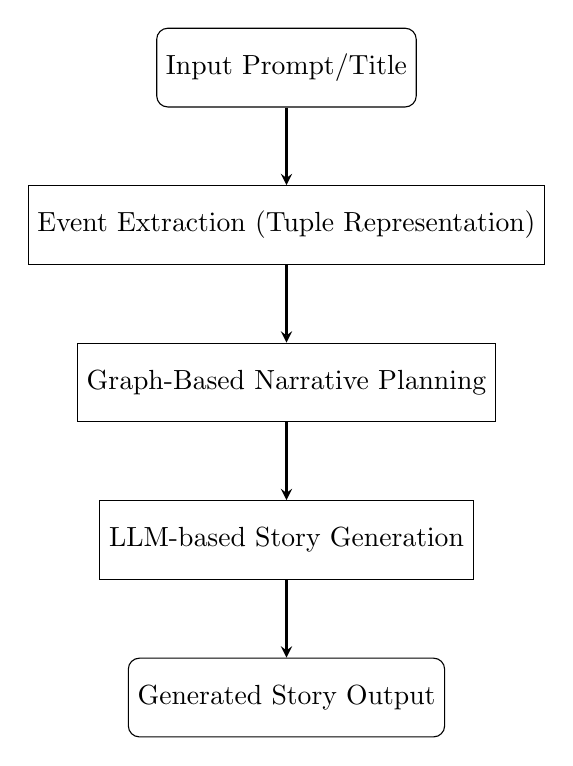
\begin{tikzpicture}[node distance=2cm]
        % Nodes
        \node (input) [startstop] {Input Prompt/Title};
        \node (eventExtraction) [process, below of=input] {Event Extraction (Tuple Representation)};
        \node (graphModeling) [process, below of=eventExtraction] {Graph-Based Narrative Planning};
        \node (llm) [process, below of=graphModeling] {LLM-based Story Generation};
        \node (output) [startstop, below of=llm] {Generated Story Output};

        % Arrows
        \draw [arrow] (input) -- (eventExtraction);
        \draw [arrow] (eventExtraction) -- (graphModeling);
        \draw [arrow] (graphModeling) -- (llm);
        \draw [arrow] (llm) -- (output);
    \end{tikzpicture}
    \caption{Workflow of the Proposed Methodology}
    \label{fig:workflow}
\end{figure}